\documentclass[a4paper]{article}
\usepackage[
				pdftex,
				colorlinks=true,
				bookmarksnumbered=true,
				bookmarksopen=true,
				bookmarksopenlevel=3,
				pdfstartview=FitP,
				urlcolor=blue,
			]{hyperref}
\pdfinfo{
			/Title(Esercitazione di Laboratorio: Circuiti con diodi)
			/Author(Coa Giulio, Licastro Dario, Montano Alessandra)
		}
\usepackage[italian]{babel}
\usepackage{geometry,titling,mdsymbol,stmaryrd,graphicx,subcaption,amsmath}
\graphicspath{{./Image/}}
\renewcommand\maketitlehooka{
								\null
								\mbox{}
								\vfill
							}
\renewcommand\maketitlehookd{
								\vfill
								\null
							}
\title{
		\begin{center}
			Esercitazione di Laboratorio:
		\end{center}
		\newline
		\begin{center}
			Circuiti con diodi
		\end{center}
	}
\author{
			Coa Giulio
			\and
			Licastro Dario
			\and
			Montano Alessandra
		}
\begin{document}
	%-----------------------------------------------------------------------------
	%  TITLE
	%-----------------------------------------------------------------------------
	\begin{titlingpage}
		\maketitle
	\end{titlingpage}
	\newpage
	%-----------------------------------------------------------------------------
	%  PURPOSE OF THE EXPERIENCE
	%-----------------------------------------------------------------------------
	\section{Scopo dell'esperienza}
		Lo scopo di questa esercitazione è analizzare vari circuiti contenenti diodi, tramite l’esecuzione di una serie di misure al fine di determinare la caratteristica statica $ I_{\mathrm{d}}(V_{\mathrm{d}}) $ dei suddetti diodi, e la successiva visualizzazione del loro comportamento con una tensione d'ingresso di tipo sinusoidale.
	%-----------------------------------------------------------------------------
	%  INSTRUMENTATION USED
	%-----------------------------------------------------------------------------
	\section{Strumentazione utilizzata}
		La strumentazione usata durante l'esercitazione è:
		\begin{center}
			\begin{tabular}{ |c|c|c| }
				\hline
				\multirow{\textbf{Strumento}}	 & \textbf{Marca e Modello} & \textbf{Caratteristiche} \\
				\hline
				\multirow{Multimetro}			 & Agilent 34401A			& \\
				\multirow{Oscilloscopio}		 & Rigol DS1054Z			& 4 canali, \\
												 &							& $ B = 50 \, \mathrm{MHz} $, \\
												 &							& $ f_{\mathrm{c}} = 1 \, \mathrm{G\frac{Sa}{s}} $, \\
												 &							& $ R_{\mathrm{i}} = 1 \, \mathrm{M\Omega} $, \\
												 &							& $ C_{\mathrm{i}} = 13 \, \mathrm{pF} $, \\
												 &							& $ 12 \, \mathrm{Mbps} $ di profondità di memoria \\
				\multirow{Generatore di segnali} & Rigol DG1022				& 2 canali, \\
												 &							& $ f_{\mathrm{uscita}} = 20 \, \mathrm{MHz} $, \\
												 &							& $ Z_{\mathrm{uscita}} = 50 \, \mathrm{\Omega} $ \\
				\multirow{Alimentatore in DC}	 & Rigol DP832				& 2 canali, \\
												 &							& $ f_{\mathrm{uscita}} = 20 \, \mathrm{MHz} $, \\
												 &							& $ Z_{\mathrm{uscita}} = 50 \, \mathrm{\Omega} $ \\
				\multirow{Sonda}				 & Rigol PVP215				& $ B = 35 \, \mathrm{MHz} $, \\
												 &							& $ V_{\mathrm{nominale}} = 300 \, \mathrm{V} $, \\
												 &							& $ L_{\mathrm{cavo}} = 1.2 \, \mathrm{m} $, \\
												 &							& $ R_{\mathrm{s}} = 1 \, \mathrm{M\Omega} $, \\
												 &							& Intervallo di compensazione: $ 10 \div 25 \, \mathrm{pF} $ \\
				\multirow{Cavi coassiali}		 &							& Capacità dell'ordine dei $ 80 \div 100 \, \mathrm{p\frac{F}{m}} $ \\
				\multirow{Connettori}			 &							& \\
				\multirow{Breadboard}			 &							& \\
				\multirow{Resistenza}			 &							& $ R = 9.9 \, \mathrm{k\Omega} $ \\
				\multirow{Diodo di Zener}		 & 1N5228					& \\
				\multirow{Diodo}				 & 1N4148					& \\
				\multirow{Condensatori}			 &							& $ C_{1} = 10 \, \mathrm{nF} $, \\
												 &							& $ C_{2} = 100 \, \mathrm{nF} $, \\
												 &							& $ C_{3} = 1 \, \mathrm{\mu F} $ \\
				\hline
			\end{tabular}
		\end{center}
	%-----------------------------------------------------------------------------
	%  THEORETICAL PREMISES
	%-----------------------------------------------------------------------------
	\section{Premesse teoriche}
		\subsection{Incertezza sulla misura dell'oscilloscopio}
			La misura del valore di un segnale tramite l’oscilloscopio (sia esso l'ampiezza, la frequenza, il periodo, etc.) presenta un'incertezza che dipende, principalmente, da due fattori:
			\begin{itemize}
				\item l’incertezza strumentale introdotta dall’oscilloscopio (ricavabile dal manuale).
				\item l’incertezza di lettura dovuta all’errore del posizionamento dei cursori.
			\end{itemize}
			Quest’ultima incertezza deriva dal fatto che il segnale visualizzato non ha uno spessore nullo sullo schermo.
		\subsection{Sonda}
			La sonda è un particolare cavo coassiale che presenta un'estremità capace di effettuare delle misurazioni.
			\newline
			Quando si usano dei classici cavi coassiali BNC-BNC al fine di collegare il circuito, su cui effettuare le misure, all'oscilloscopio, si sta inserendo in parallelo al circuito un condensatore di capacità ($ C_{\mathrm{c}} $) pari a quella del cavo.
			\begin{figure}[h!]
				\centering
				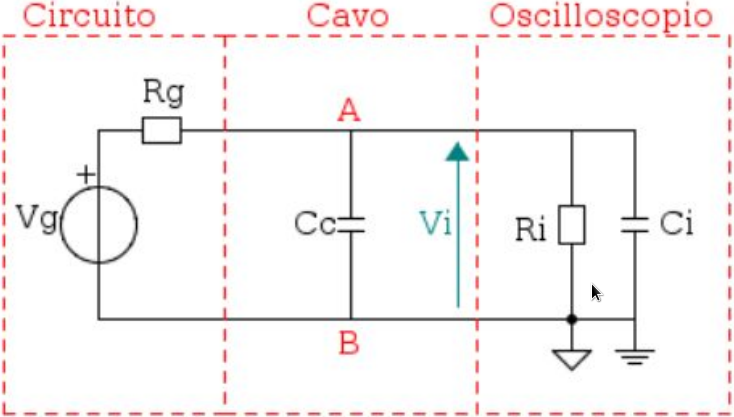
\includegraphics[scale=0.4]{theveninCavoDSO}
				\caption{Circuito analizzato collegato all'oscilloscopio tramite un cavo coassiale BNC-BNC.}
				\label{fig:theveninCavoDSO}
			\end{figure}
			\newline
			In questo caso, l’oscilloscopio si comporta, in ingresso, come un filtro passa-basso con una frequenza di taglio ($ f = \frac{1}{2\pi R_{i} (C_{s} + C_{i})} $). L'uso di una sonda per misurare delle grandezze in un circuito, si può vedere come l'inserimento di un condensatore in serie al circuito.
			\begin{figure}[h!]
				\centering
				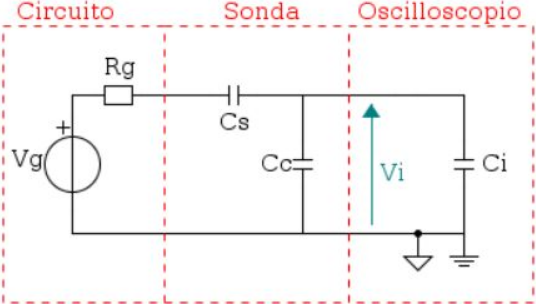
\includegraphics[scale=0.4]{theveninSondaDSOCircuito}
				\caption{Circuito analizzato collegato all'oscilloscopio tramite una sonda.}
				\label{fig:theveninSondaDSOCircuito}
			\end{figure}
			\newpage
			L'introduzione di questo condensatore comporta un calo della capacità equivalente vista all'ingresso del circuito ($ \mathrm{\frac{C_{s} (C_{c} + C_{i})}{C_{s} + C_{c} + C_{i}} \ll C_{c} + C_{i}} $), ovvero una riduzione della frequenza del polo ($ f_{\mathrm{polo}} = \frac{1}{2\pi R_{i} (C_{s} + C_{i})} $); ciò porta ad una perdita d'informazioni in bassa frequenza.
			\newline
			Al fine di evitare tale perdita d'informazioni, si pone, in parallelo al condensatore, una resistenza.
			\begin{figure}[h!]
				\centering
				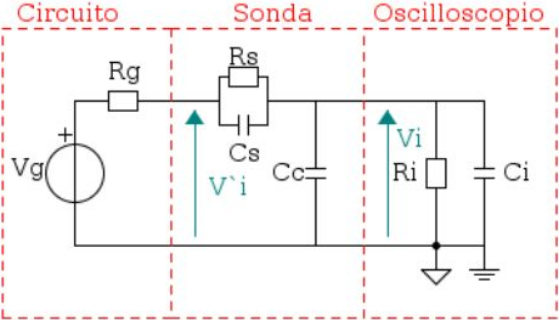
\includegraphics[scale=0.4]{theveninSondaDSOResistenza}
				\caption{Circuito analizzato collegato all'oscilloscopio tramite una sonda.}
				\label{fig:theveninSondaDSOResistenza}
			\end{figure}
			\newline
			Tale resistenza comporta la presenza di uno zero, oltre al polo precedentemente detto.
			\begin{figure}[h!]
				\centering
				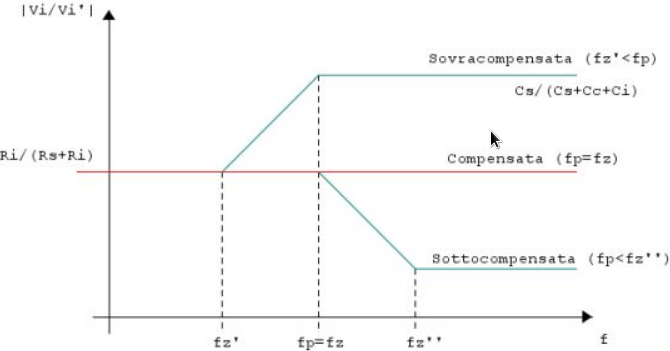
\includegraphics[scale=0.4]{sondaBode}
				\caption{Diagramma di Bode della funzione di trasferimento del circuito.}
				\label{fig:sondaBode}
			\end{figure}
			\newpage
			A seconda dell'elevata o della bassa compensazione della sonda, il segnale sarà distorto verso l'alto o verso il basso.
			\begin{figure}[h!]
				\centering
				\begin{subfigure}{0.4\textwidth}
					\centering
					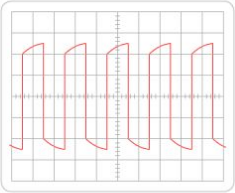
\includegraphics[scale=0.5]{sondaSegnaleSottocompensato}
					\caption{Sonda sottocompensata.}
				\end{subfigure}
				\begin{subfigure}{0.4\textwidth}
					\centering
					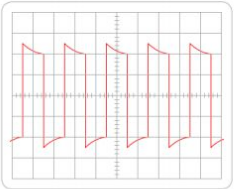
\includegraphics[scale=0.5]{sondaSegnaleSovracompensato}
					\caption{Sonda sovracompensata.}
				\end{subfigure}
				\caption{Visualizzazione del segnale al variare della compensazione della sonda.}
				\label{fig:sondaSegnaleNonCompensato}
			\end{figure}
			\newline
			La sonda risulta compensata quando la frequenza del polo coincide con la frequenza dello zero; ciò avviene quando $ R_{\mathrm{s}} C_{\mathrm{s}} = R_{\mathrm{i}} (C_{\mathrm{c}} + C_{\mathrm{i}})} $. La sonda presenta un opportuno trimmer che influenza il valore di $ R_{\mathrm{s}} $ e permette la compensazione. Al fine di verificare se la sonda è compensata si esegue un confronto con un segnale noto.
			\begin{figure}[h!]
				\centering
				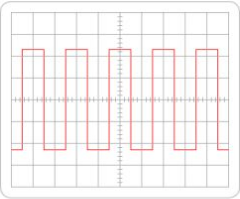
\includegraphics[scale=0.5]{sondaSegnaleCompensato}
				\caption{Sonda compensata.}
				\label{fig:sondaSegnaleCompensato}
			\end{figure}
		\subsection{Diodo}
			Il diodo è un bipolo non lineare il cui comportamento è descritto dalle due seguenti espressioni analitiche equivalenti tra loro
			\newline
			\begin{center}
				$ i_{\mathrm{D}} = I_{\mathrm{S}} \cdot (e^{\mathrm{\frac{v_{\mathrm{D}}}{\eta \cdot V_{\mathrm{T}}}}} - 1) $
			\end{center}
			\newline
			\begin{center}
				$ v_{\mathrm{D}} = \eta \cdot V_{\mathrm{T}} \cdot \ln (\frac{i_{\mathrm{D}}}{I_{\mathrm{S}}} + 1) $
			\end{center}
			dove $ V_{\mathrm{T}} $ è la tensione termica del diodo ($ V_{\mathrm{T}} = \frac{\mathrm{k \cdot T}}{\mathrm{q}} $), $ I_{\mathrm{S}} $ è la corrente di saturazione ed $ \eta $ è il fattore di non idealità.
			\begin{figure}[h!]
				\centering
				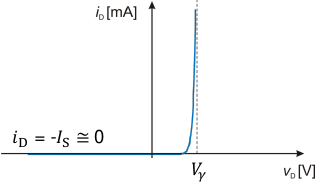
\includegraphics[scale=0.7]{caratteristicaStatica}
				\caption{Caratteristica statica di un diodo.}
				\label{fig:caratteristicaStatica}
			\end{figure}
			\newpage
			Si noti come, al crescere di $ v_{\mathrm{D}} $, la corrente $ i_{\mathrm{D}} $, ovvero la corrente che attaversa il diodo, aumenti (regione di polarizzazione); in particolare, dopo il raggiungimento della tensione di soglia $ V_{\mathrm{\gamma}} $, il diodo tende a comportarsi come un generatore ideale indipendente di tensione di valore pari a $ V_{\mathrm{\gamma}} $.
			\newline
			Al contrario, quando $ v_{\mathrm{D}} $ è troppo bassa, la corrente $ i_{\mathrm{D}} $ è pari a $ -I_{\mathrm{S}} $, ovvero circa nulla; ciò porta il diodo a comportarsi similmente ad un circuito aperto (regione di polarizzazione inversa). Questa condizione può dare luogo al fenomeno del breakdown, ovvero quando il diodo conduce in direzione opposta; tale fenomeno porta, solitamente, alla rottura del diodo.
			\subsubsection{Diodo di Zener}
				Sono particolari tipi di diodi progettati appositamente per lavorare anche in polarizzazione inversa; questi diodi non si rompono se si verifica il breakdown, anzi sono caratterizzati da una tensione di soglia negativa, detta, per l'appunto, tensione di breakdown.
				\begin{figure}[h!]
					\centering
					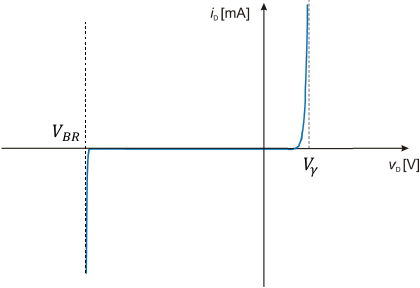
\includegraphics[scale=0.7]{caratteristicaStaticaDiodoZener}
					\caption{Caratteristica statica di un diodo di Zener.}
					\label{fig:caratteristicaStaticaDiodoZener}
				\end{figure}
		\subsection{Raddrizzatore a semplice semionda}
			Il raddrizzatore a semplice semionda è un circuito che, data una tensione in input, caratterizzata da un valor medio non nullo, ne estrae la parte positiva; il segnale in uscita presenta valor medio nullo.
			\begin{equation*}
				v_{\mathrm{out}} =
				\begin{cases}
					v_{\mathrm{in}} & v_{\mathrm{in}} > 0 \\
					0 				& v_{\mathrm{in}} \le 0
				\end{cases}
			\end{equation*}
			\begin{figure}[h!]
				\centering
				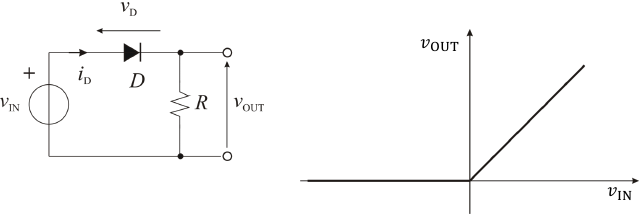
\includegraphics[scale=0.7]{transcaratteristicaStaticaRaddrizzatoreASempliceSemionda}
				\caption{Circuito e transcaratteristica statica di un raddrizzatore a semplice semionda.}
				\label{fig:transcaratteristicaStaticaRaddrizzatoreASempliceSemionda}
			\end{figure}
		\subsection{Rivelatore di picco}
			Il rivelatore di picco è un circuito che, dato un segnale in ingresso, ne determina il valore di picco.
			\newline
			\begin{center}
				$ v_{\mathrm{in}} = V_{\mathrm{p}} \cdot \sin(2 \pi \cdot f \cdot t) $
			\end{center}
			\newline
			\begin{center}
				$ v_{\mathrm{out}} = V_{\mathrm{p}} $
			\end{center}
			\begin{figure}[h!]
				\centering
				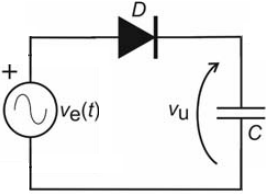
\includegraphics[scale=0.7]{rivelatoreDiPiccoCircuito}
				\caption{Circuito del rivelatore di picco.}
				\label{fig:rivelatoreDiPiccoCircuito}
			\end{figure}
		\subsection{Protezione ESD}
			La protezione ESD è un circuito usato come protezione da scariche elettrostatiche, caratterizzato dall'imposizione di una tensione massima e di una tensione minima.
			\begin{equation*}
				v_{\mathrm{out}} =
				\begin{cases}
					-V_{\mathrm{\gamma}}				  & v_{\mathrm{in}} < -V_{\mathrm{\gamma}} \\
					v_{\mathrm{in}} 				 	  & -V_{\mathrm{\gamma}} \le v_{\mathrm{in}} \le V_{\mathrm{DD}} + V_{\mathrm{\gamma}} \\
					V_{\mathrm{DD}} + V_{\mathrm{\gamma}} & v_{\mathrm{in}} > V_{\mathrm{DD}} + V_{\mathrm{\gamma}}
				\end{cases}
			\end{equation*}
			\begin{figure}[h!]
				\centering
				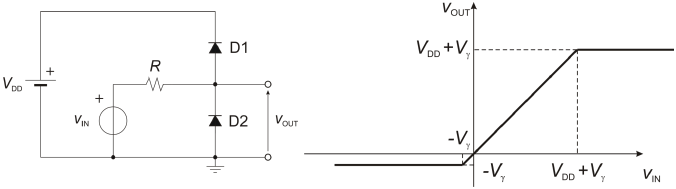
\includegraphics[scale=0.7]{transcaratteristicaStaticaProtezioneESD}
				\caption{Circuito e transcaratteristica statica di una protezione ESD.}
				\label{fig:transcaratteristicaStaticaProtezioneESD}
			\end{figure}
	%-----------------------------------------------------------------------------
	%  LABORATORY EXPERIENCE
	%-----------------------------------------------------------------------------
	\section{Esperienza in laboratorio}
		\subsection{Caratteristiche statiche}
			Abbiamo montato sulla breadboard la resistenza, il diodo D=1N4148 e l'elemento di collegamento seguendo lo schema in figura.
			\begin{figure}[h!]
				\centering
				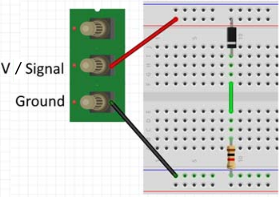
\includegraphics[scale=0.7]{caratteristicheStaticheCircuito}
				\caption{Circuito.}
				\label{fig:caratteristicheStaticheCircuito}
			\end{figure}
			\newline
			Successivamente, per mezzo del multimetro, abbiamo misurato la resistenza, verificando che tale valore rientri nel $ 5 \% $ di tolleranza dato dal costruttore. Dopo aver alimentato, collegando la breadboard all'alimentatore in DC per mezzo di due cavi a banana, il circuito, abbiamo variato la tensione in ingresso secondo i valori fornitici, misurando, sempre tramite il multimetro, i valori di tensione ai capi della resistenza.
			\newline
			In seguito abbiamo connesso alla breadboard, al posto dell'alimentatore in DC, il generatore di segnali tramite un cavo coassiale BNC-banana, impostandolo per fornire un segnale d'ampiezza $ V_{\mathrm{pp}} = 10 \, \mathrm{V} $ e frequenza $ f = 1 \, \mathrm{kHz} $, ed, al posto del multimetro, l'oscilloscopio tramite due sonde.
			\newline
			Infine, abbiamo sostituito il diodo con il diodo di Zener D=1N5228 e ripetuto l'esperienza.
		\subsection{Raddrizzatore a semplice semionda}
			Dopo aver realizzato il circuito richiesto, collegando un condensatore in parallelo al circuito e sostituendo il diodo di Zener con il diodo usato precedentemente, si è proceduto col misurare l'ampiezza $ V_{\mathrm{pp}} $ del segnale al variare della capacità del condensatore.
			\begin{figure}[h!]
				\centering
				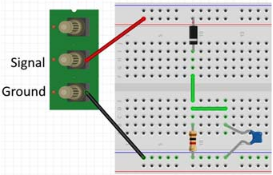
\includegraphics[scale=0.7]{raddrizzatoreASempliceSemiondaCircuito}
				\caption{Circuito.}
				\label{fig:raddrizzatoreASempliceSemiondaCircuito}
			\end{figure}
			\newpage
			In questo modo, si è potuto apprezzare come la capacità del condensatore influenzi il segnale in uscita; infine, si è sostituito il diodo con il diodo di Zener e ripetuto l'esperienza.
		\subsection{Rivelatore di picco}
			Abbiamo posizionato gli elementi circuitali sulla breadboard in modo da costruire il rivelatore di picco, connettendo, tramite due sonde, l'ingresso e l'uscita all'oscilloscopio ed abbiamo impostato il generatore di segnali di modo da visualizzare un segnale sinusoidale d'ampiezza $ V_{\mathrm{pp}} = 10 \, \mathrm{V} $ e frequenza $ f = 1 \, \mathrm{kHz} $.
			\newline
			In tal modo, in uscita, visualizziamo un segnale costante sul valore di picco del segnale in ingresso; come si può vedere dalle immagini, tale fenomeno è indipendente dalla capacità del condensatore usato.
			\begin{figure}[h!]
				\centering
				\begin{subfigure}{0.4\textwidth}
					\centering
					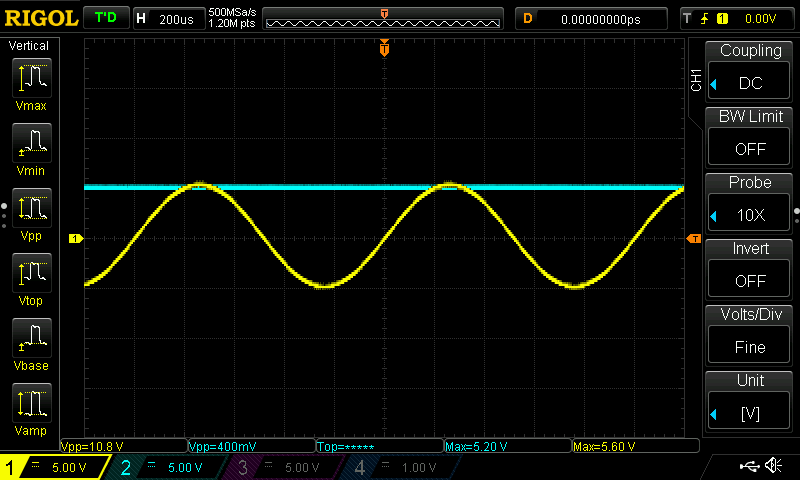
\includegraphics[scale=0.2]{rivelatoreDiPicco10n}
					\caption{Rivelatore di picco con il condensatore da $ 10 \, \mathrm{nF} $.}
				\end{subfigure}
				\begin{subfigure}{0.4\textwidth}
					\centering
					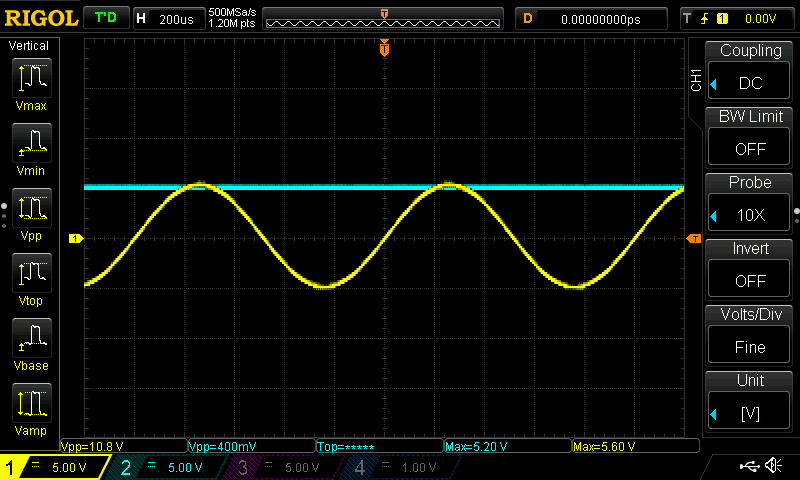
\includegraphics[scale=0.2]{rivelatoreDiPicco100n}
					\caption{Rivelatore di picco con il condensatore da $ 100 \, \mathrm{nF} $.}
				\end{subfigure}
				\begin{subfigure}{1\textwidth}
					\centering
					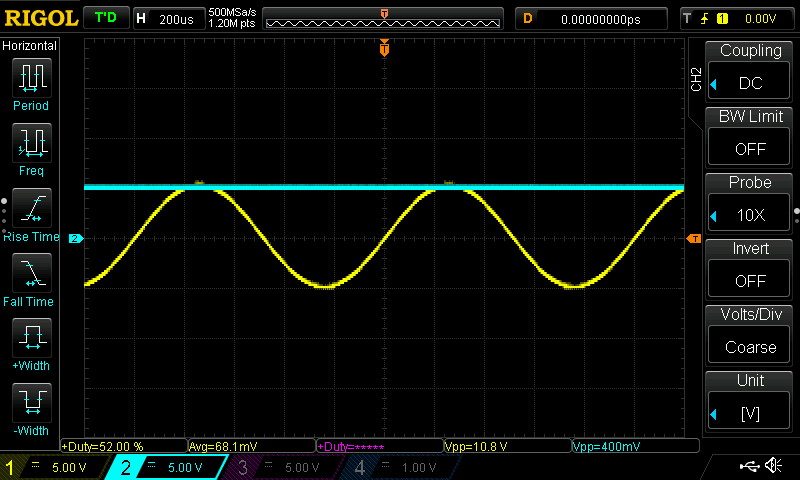
\includegraphics[scale=0.4]{rivelatoreDiPicco1micro}
					\caption{Rivelatore di picco con il condensatore da $ 1 \, \mathrm{\mu F} $.}
				\end{subfigure}
				\label{fig:rivelatoreDiPicco}
			\end{figure}
			\newpage
			Ciò avviene poichè, una volta alimentato il circuito, il condensatore inizia a caricarsi, raggiungendo il valore di picco del segnale in ingresso; a tal punto, il segnale inizia la "fase di discesa", dove diminuisce la sua ampiezza.
			\newline
			Il diodo, analizzato in condizioni di ampio segnale, si comporta come un circuito aperto per ogni valore di tensione $ v_{\mathrm{D}} $ inferiore alla tensione di soglia $ V_{\mathrm{\gamma}} $; ciò implica che, quando il segnale dimuinisce la sua ampiezza, il diodo smette di condurre corrente in quanto la tensione $ v_{\mathrm{D}} $ diventa inferiore alla tensione di soglia.
			\newline
			Questo evento comporta l'impossibilità, da parte del condensatore, della fase di scarica, per cui esso preserverà la tensione di picco del segnale in ingresso.
			Data la non-immediatezza del calo di tensione, esiste un momento in cui il segnale diminuisce la sua ampiezza, ma essa rimane superiore alla tensione di soglia del diodo; in tale momento il condensatore effettua una breve fase di scarica, che porta ad un errore nel funzionamento del circuito, in quanto il valore "memorizzato" non è quello della tensione di picco, ma uno leggermente inferiore.
		\subsection{Circuito per la protezione da scariche elettrostatiche}
			Abbiamo posizionato gli elementi circuitali sulla breadboard in modo da costruire la protezione ESD; in questo modo, in uscita, visualizziamo un segnale che presenta i valori di picco limitati, di cui abbiamo determinato $ V_{\mathrm{min}} $ e $ V_{\mathrm{max}} $.
			\begin{figure}[h!]
				\centering
				\begin{subfigure}{0.4\textwidth}
					\centering
					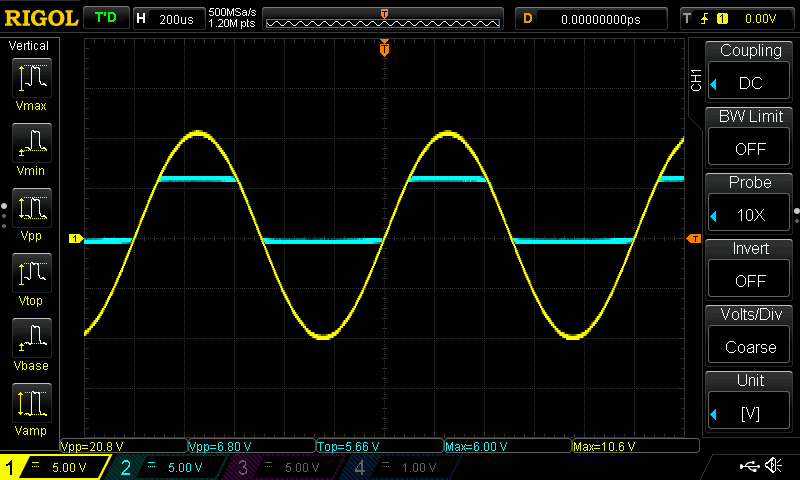
\includegraphics[scale=0.2]{protezioneESD}
					\caption{Protezione ESD.}
				\end{subfigure}
				\begin{subfigure}{0.4\textwidth}
					\centering
					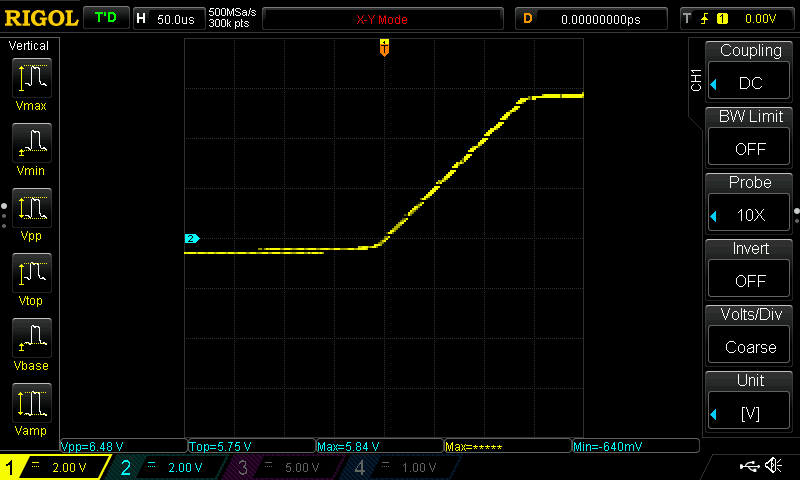
\includegraphics[scale=0.2]{protezioneESDTranscaratteristica}
					\caption{Transcaratteristica della protezione ESD.}
				\end{subfigure}
				\label{fig:protezioneESD}
			\end{figure}
	%-----------------------------------------------------------------------------
	%  RESULTS
	%-----------------------------------------------------------------------------
	\section{Risultati}
		\subsection{Caratteristiche statiche}
			\subsubsection{Diodo}
				I risultati ottenuti al variare della tensione in ingresso, fornita con l'alimentatore, sono stati riportati nella seguente tabella.
				\begin{center}
					\begin{tabular}{ |c|c|c| }
						\hline
						\multirow{\textbf{$ V_{\mathrm{e}} $ [$ \mathrm{V} $]}}	 & \textbf{$ V_{\mathrm{u}} $} & \textbf{$ I_{\mathrm{D}} $} \\
						\hline
						\multirow{$ -4 $}										 & $ -3.31 \, \mathrm{mV} $   & $ -4.65 \, \mathrm{nA} $ \\
						\multirow{$ -3.5 $}										 & $ -2.81 \, \mathrm{mV} $   & $ -4.34 \, \mathrm{nA} $ \\
						\multirow{$ -3 $}										 & $ -2.32 \, \mathrm{mV} $   & $ -3.84 \, \mathrm{nA} $ \\
						\multirow{$ -2 $}										 & $ -1.33 \, \mathrm{mV} $   & $ -3.23 \, \mathrm{nA} $ \\
						\multirow{$ -1 $}										 & $ -0.37 \, \mathrm{mV} $   & $ -2.73 \, \mathrm{nA} $ \\
						\multirow{$ 0 $}										 & $ 0.006 \, \mathrm{mV} $	  & $ 101 \, \mathrm{pA} $ \\
						\multirow{$ 0.2 $}										 & $ 0.019 \, \mathrm{mV} $   & $ 209 \, \mathrm{nA} $ \\
						\multirow{$ 0.4 $}										 & $ 0.966 \, \mathrm{mV} $   & $ 4.58 \, \mathrm{\mu A} $ \\
						\multirow{$ 0.6 $}										 & $ 43.5 \, \mathrm{mV} $    & $ 17.9 \, \mathrm{\mu A} $ \\
						\multirow{$ 0.8 $}										 & $ 191 \, \mathrm{mV} $     & $ 34.7 \, \mathrm{\mu A} $ \\
						\multirow{$ 1 $}										 & $ 373 \, \mathrm{mV} $     & $ 53.1 \, \mathrm{\mu A} $ \\
						\multirow{$ 1.5 $}										 & $ 847 \, \mathrm{mV} $     & $ 101 \, \mathrm{\mu A} $ \\
						\multirow{$ 2 $}										 & $ 1.33 \, \mathrm{V} $     & $ 149 \, \mathrm{\mu A} $ \\
						\hline
					\end{tabular}
				\end{center}
				Si può notare che il diodo utilizzato non è adatto all'uso in polarizzazione inversa, infatti, per valori di $ V_{\mathrm{e}} $ negativi, otteniamo valori di $ V_{\mathrm{u}} $ molto bassi, che si mantengono intorno allo zero. Come si può intuire dai valori misurati, la tensione di soglia $ V_{\mathrm{\gamma}} $ è pari a $ 600 \, \mathrm{mV} $.
				\begin{figure}[h!]
					\centering
					\begin{subfigure}{0.5\textwidth}
						\centering
						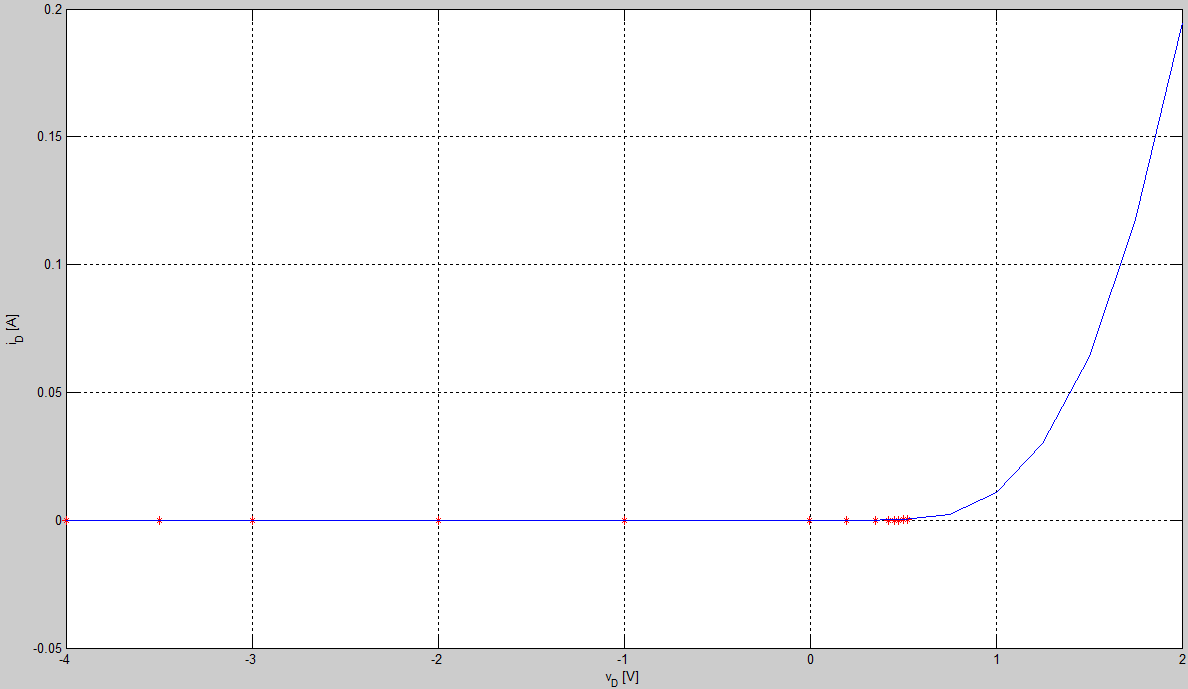
\includegraphics[scale=0.2]{caratteristicheStaticheDiodoCaratteristica}
						\caption{Caratteristica statica del diodo.}
					\end{subfigure}
					\begin{subfigure}{0.3\textwidth}
						\centering
						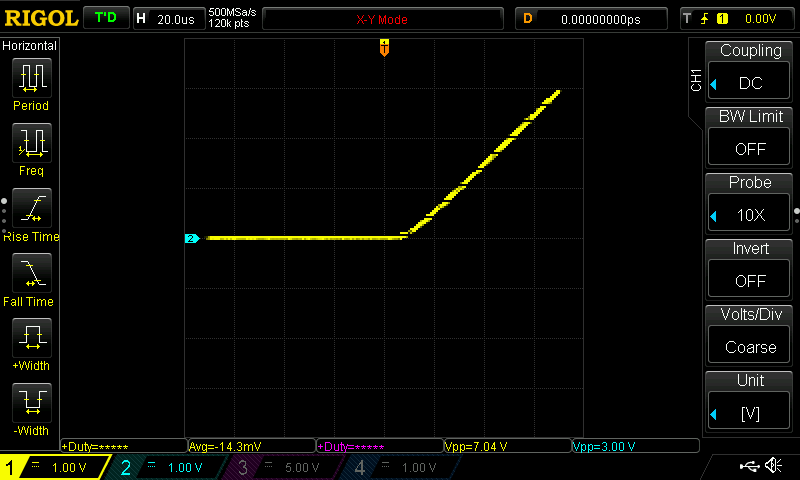
\includegraphics[scale=0.2]{caratteristicheStaticheDiodoTranscaratteristica}
						\caption{Transcaratteristica statica del diodo.}
					\end{subfigure}
					\label{fig:caratteristicheStaticheDiodo}
				\end{figure}
				\newline
				Dopo aver connesso il generatore di segnali, la sonda e l'oscilloscopio  come illustrato precedentemente, abbiamo ottenuto la seguente immagine, dove l'output è distorto per effetto del circuito; in particolare, la parte dove il segnale assume valori negativi è stata azzerata e la parte dove il segnale assume valori positivi è stata attenuata a causa della non idealità del diodo.
				\begin{figure}[h!]
					\centering
					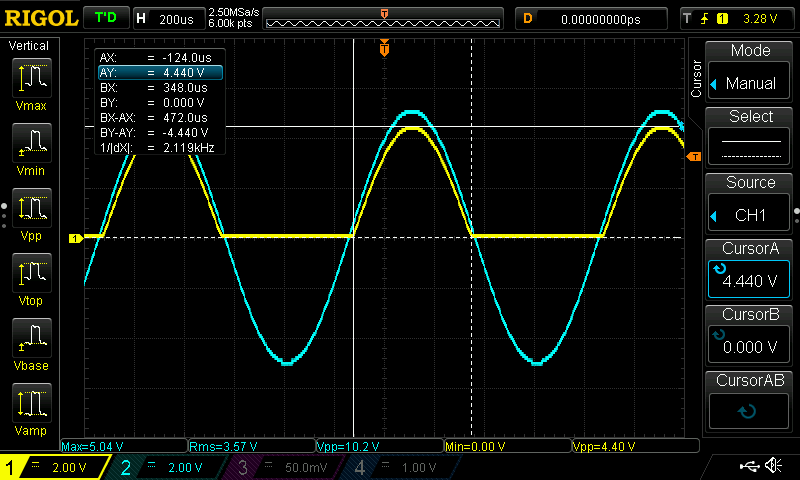
\includegraphics[scale=0.5]{ampiezzaDiPiccoDiodo}
					\caption{Segnale originale e segnale prelevato a valle del diodo.}
					\label{fig:ampiezzaDiPiccoDiodo}
				\end{figure}
				\newline
				In seguito, abbiamo misurato l'ampiezza di picco del segnale in output, ottenendo $ 4.40 \, \mathrm{V} $.
			\subsubsection{Diodo di Zener}
				Dopo aver eseguito un'altra volta la procedura utilizzando il diodo di Zener, abbiamo ottenuto dei valori per tensioni negative in input che sono coerenti con la definizione di diodo di Zener.
				\begin{center}
					\begin{tabular}{ |c|c|c| }
						\hline
						\multirow{\textbf{$ V_{\mathrm{e}} $ [$ \mathrm{V} $]}}	 & \textbf{$ V_{\mathrm{u}} $} & \textbf{$ I_{\mathrm{D}} $} \\
						\hline
						\multirow{$ -4 $}										 & $ -3.31 \, \mathrm{mV} $   & $ -0.334 \, \mathrm{\mu A} $ \\
						\multirow{$ -3.5 $}										 & $ -2.81 \, \mathrm{mV} $   & $ -0.284 \, \mathrm{\mu A} $ \\
						\multirow{$ -3 $}										 & $ -2.32 \, \mathrm{mV} $   & $ -0.234 \, \mathrm{\mu A} $ \\
						\multirow{$ -2 $}										 & $ -1.33 \, \mathrm{mV} $   & $ -0.134 \, \mathrm{\mu A} $ \\
						\multirow{$ -1 $}										 & $ -0.37 \, \mathrm{mV} $   & $ -37.4 \, \mathrm{nA} $ \\
						\multirow{$ 0 $}										 & $ 0.006 \, \mathrm{mV} $	  & $ 606 \, \mathrm{pA} $ \\
						\multirow{$ 0.2 $}										 & $ 0.019 \, \mathrm{mV} $   & $ 1.92 \, \mathrm{nA} $ \\
						\multirow{$ 0.4 $}										 & $ 0.966 \, \mathrm{mV} $   & $ 97.6 \, \mathrm{nA} $ \\
						\multirow{$ 0.6 $}										 & $ 43.5 \, \mathrm{mV} $    & $ 4.39 \, \mathrm{\mu A} $ \\
						\multirow{$ 0.8 $}										 & $ 191 \, \mathrm{mV} $     & $ 19.2 \, \mathrm{\mu A} $ \\
						\multirow{$ 1 $}										 & $ 373 \, \mathrm{mV} $     & $ 37.7 \, \mathrm{\mu A} $ \\
						\multirow{$ 1.5 $}										 & $ 847 \, \mathrm{mV} $     & $ 85.6 \, \mathrm{\mu A} $ \\
						\multirow{$ 2 $}										 & $ 1.33 \, \mathrm{V} $     & $ 134 \, \mathrm{\mu A} $ \\
						\hline
					\end{tabular}
				\end{center}
				Come si può intuire dai valori misurati, la tensione di soglia $ V_{\mathrm{\gamma}} $ è pari a $ 600 \, \mathrm{mV} $, mentre la tensione di breakdown $ V_{\mathrm{br}} $ è pari a $ -1 \, \mathrm{V} $.
				\begin{figure}[h!]
					\centering
					\begin{subfigure}{0.5\textwidth}
						\centering
						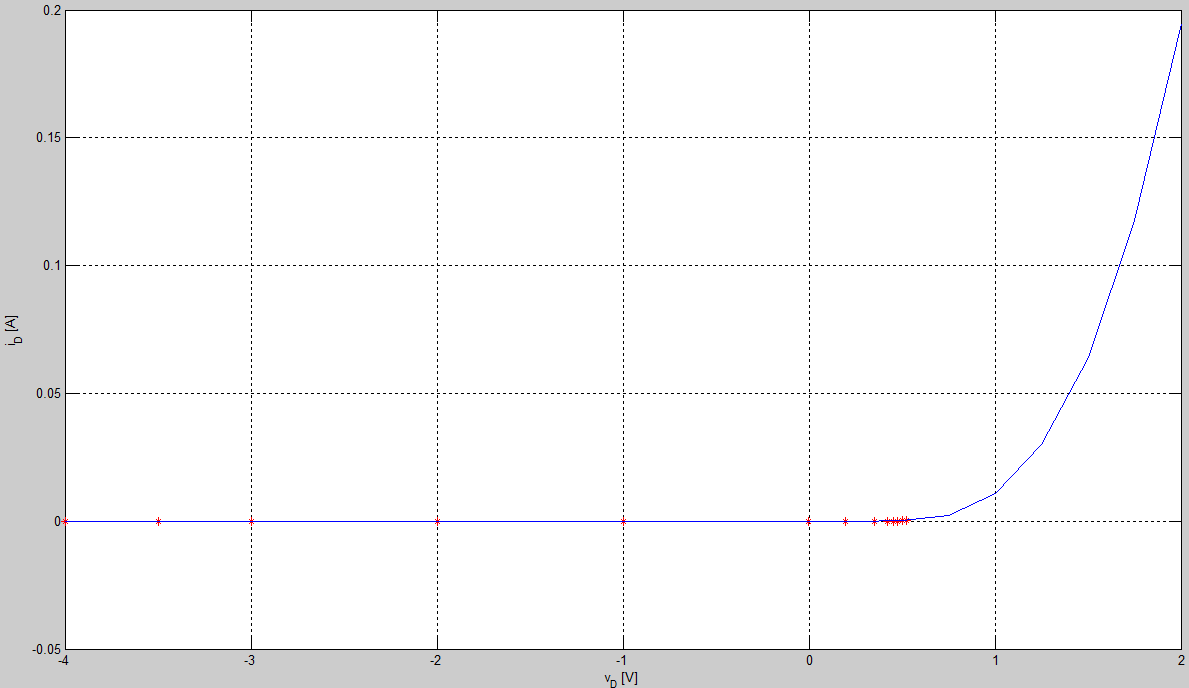
\includegraphics[scale=0.2]{caratteristicheStaticheDiodoDiZenerCaratteristica}
						\caption{Caratteristica statica del diodo di Zener.}
					\end{subfigure}
					\begin{subfigure}{0.3\textwidth}
						\centering
						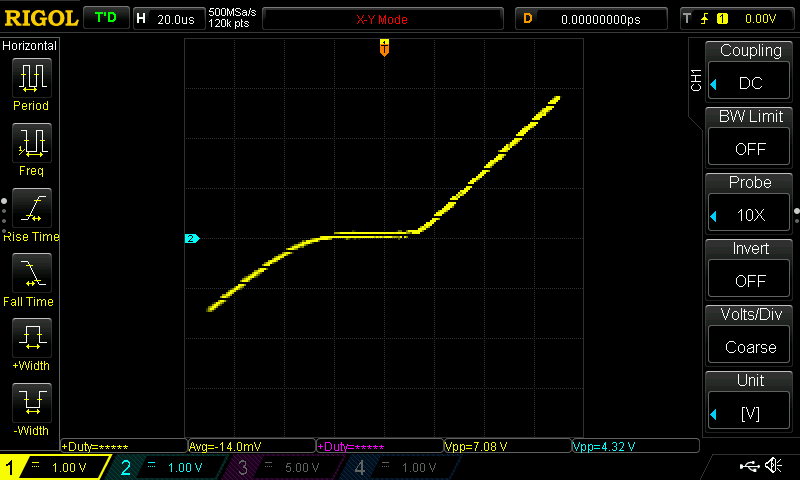
\includegraphics[scale=0.2]{caratteristicheStaticheDiodoDiZenerTranscaratteristica}
						\caption{Transcaratteristica statica del diodo di Zener.}
					\end{subfigure}
					\label{fig:caratteristicheStaticheDiodoDiZener}
				\end{figure}
				\newline
				A differenza del diodo usato in precedenza, il diodo di Zener, proprio perchè adatto a lavorare in polarizzazione inversa, conduce anche per valori di tensione negativi, portandoci ad osservare il seguente segnale.		
				\begin{figure}[h!]
					\centering
					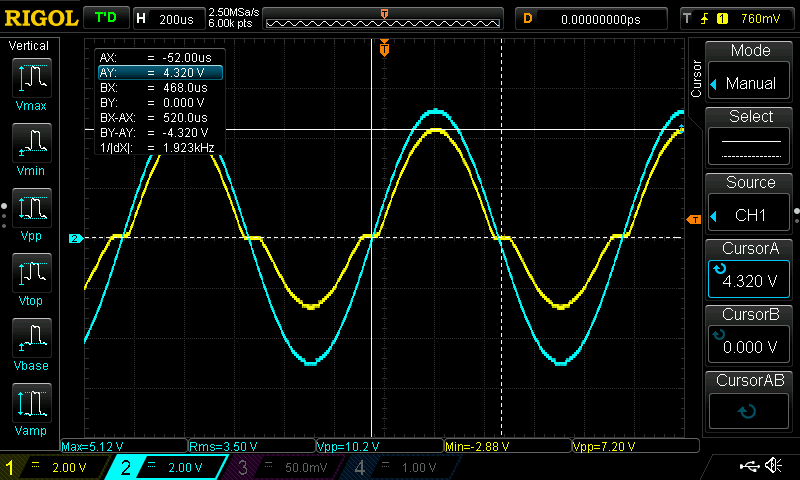
\includegraphics[scale=0.5]{ampiezzaDiPiccoDiodoDiZener}
					\caption{Segnale originale e segnale prelevato a valle del diodo di Zener.}
					\label{fig:ampiezzaDiPiccoDiodoDiZener}
				\end{figure}
				\newline
				Come fatto in precedenza, abbiamo misurato l'ampiezza di picco del segnale in output, ottenendo $ 4.32 \, \mathrm{V} $.
		\subsection{Raddrizzatore a semplice semionda}
			\subsubsection{Diodo}
				Abbiamo costruito il circuito usando i vari condensatori, misurando, ogni volta, l'ampiezza $ V_{\mathrm{pp}} $ del segnale in output.
				\begin{center}
					\begin{tabular}{ |c|c|c| }
						\hline
						\multirow{\textbf{$ C_{1} $}} & \textbf{$ C_{2} $} & \textbf{$ C_{3} $} \\
						\hline
						\multirow{$ 4.56 \, \mathrm{V} $} & $ 2.56 \, \mathrm{V} $ & $ 480 \, \mathrm{mV} $ \\
						\hline
					\end{tabular}
				\end{center}
				\begin{figure}[h!]
					\centering
					\begin{subfigure}{0.4\textwidth}
						\centering
						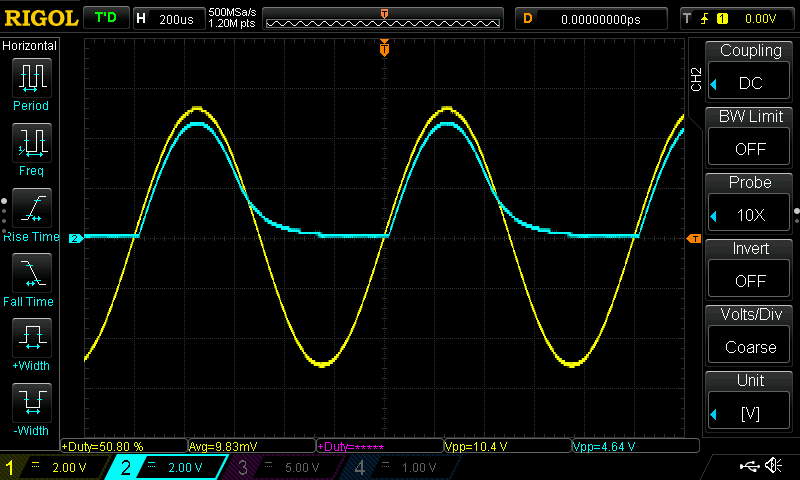
\includegraphics[scale=0.2]{raddrizzatoreASempliceSemiondaDiodo10n}
						\caption{Raddrizzatore a semplice semionda con il condensatore da $ 10 \, \mathrm{nF} $.}
					\end{subfigure}
					\begin{subfigure}{0.4\textwidth}
						\centering
						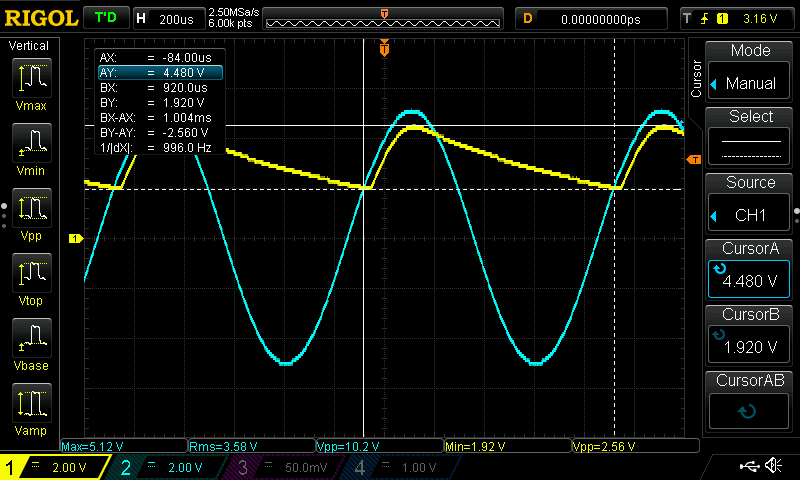
\includegraphics[scale=0.2]{raddrizzatoreASempliceSemiondaDiodo100n}
						\caption{Raddrizzatore a semplice semionda con il condensatore da $ 100 \, \mathrm{nF} $.}
					\end{subfigure}
					\begin{subfigure}{1\textwidth}
						\centering
						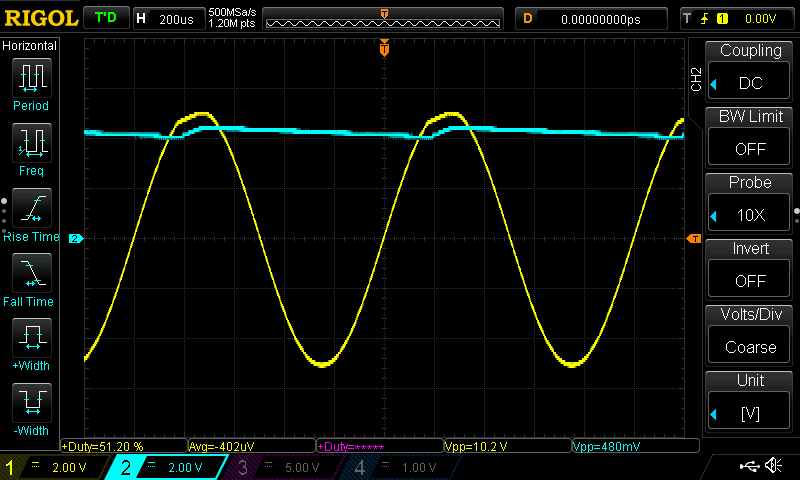
\includegraphics[scale=0.4]{raddrizzatoreASempliceSemiondaDiodo1micro}
						\caption{Raddrizzatore a semplice semionda con il condensatore da $ 1 \, \mathrm{\mu F} $.}
					\end{subfigure}
					\label{fig:raddrizzatoreASempliceSemiondaDiodo}
				\end{figure}
				\newline
				Possiamo notare come, al decrescere della capacità del condensatore, aumenti l'ampiezza $ V_{\mathrm{pp}} $ del segnale in output, ovvero come il segnale in input viene distorto sempre di più.
			\subsubsection{Diodo di Zener}	
				Successivamente, abbiamo sostituito il diodo con il diodo di Zener, ripetendo l'intera esperienza.
				\begin{center}
					\begin{tabular}{ |c|c|c| }
						\hline
						\multirow{\textbf{$ C_{1} $}} & \textbf{$ C_{2} $} & \textbf{$ C_{3} $} \\
						\hline
						\multirow{$ 7.36 \, \mathrm{V} $} & $ 7.12 \, \mathrm{V} $ & $ 5.68 \, \mathrm{V} $ \\
						\hline
					\end{tabular}
				\end{center}
				\begin{figure}[h!]
					\centering
					\begin{subfigure}{0.4\textwidth}
						\centering
						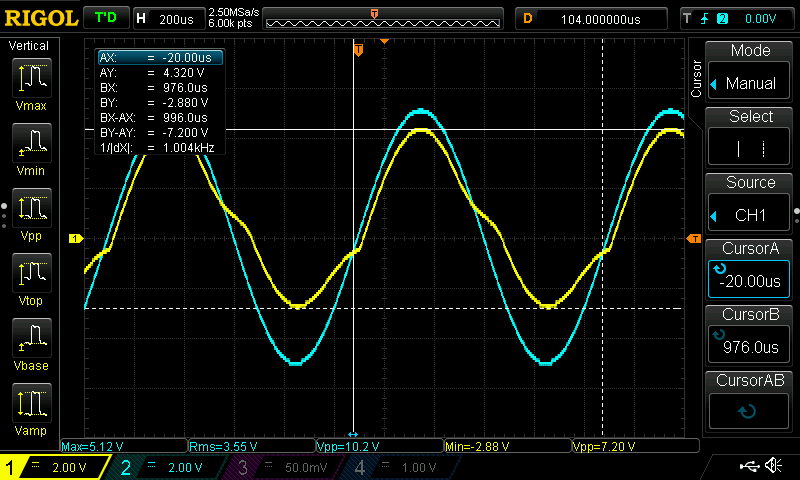
\includegraphics[scale=0.2]{raddrizzatoreASempliceSemiondaDiodoDiZener10n}
						\caption{Raddrizzatore a semplice semionda con il condensatore da $ 10 \, \mathrm{nF} $.}
					\end{subfigure}
					\begin{subfigure}{0.4\textwidth}
						\centering
						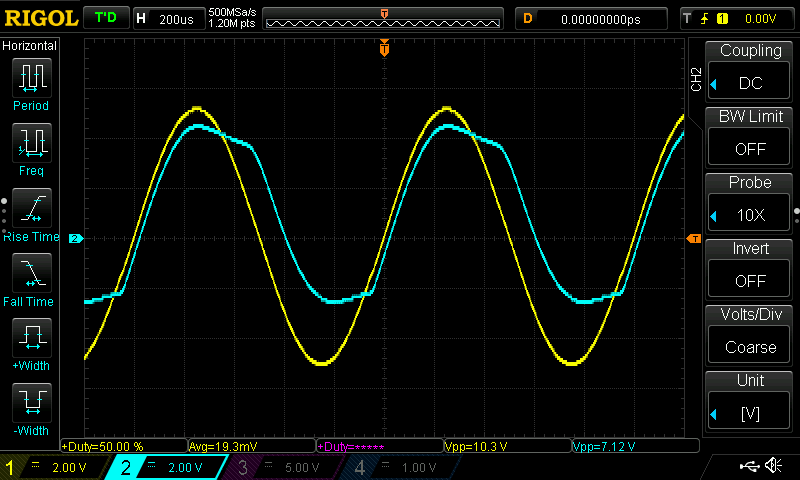
\includegraphics[scale=0.2]{raddrizzatoreASempliceSemiondaDiodoDiZener100n}
						\caption{Raddrizzatore a semplice semionda con il condensatore da $ 100 \, \mathrm{nF} $.}
					\end{subfigure}
					\begin{subfigure}{1\textwidth}
						\centering
						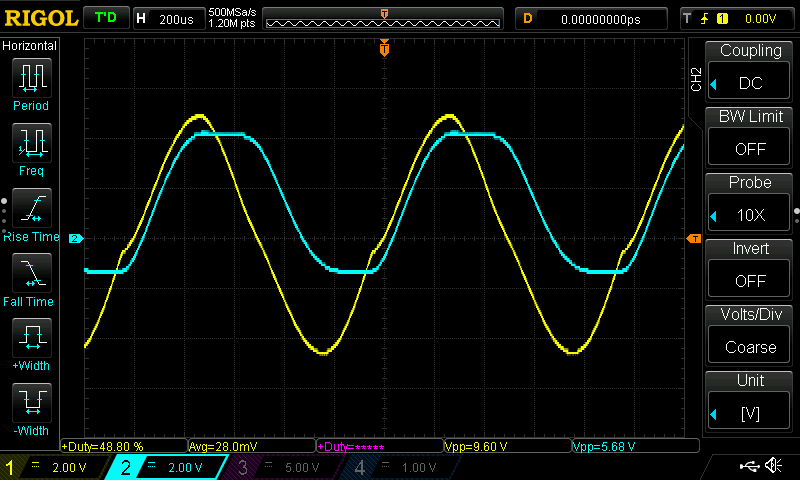
\includegraphics[scale=0.3]{raddrizzatoreASempliceSemiondaDiodoDiZener1micro}
						\caption{Raddrizzatore a semplice semionda con il condensatore da $ 1 \, \mathrm{\mu F} $.}
					\end{subfigure}
					\label{fig:raddrizzatoreASempliceSemiondaDiodoDiZener}
				\end{figure}
				\newpage
				Possiamo notare come, anche in questo caso, al decrescere della capacità del condensatore, aumenti l'ampiezza $ V_{\mathrm{pp}} $ del segnale in output.
				\newline
				Infine abbiamo riposizionato il diodo D=1N4148, lasciando montato il condensatore da $ 1 \, \mathrm{\mu F} $ e connettendo al circuito il generatore di segnali impostato al fine di avere un'ampiezza $ V_{\mathrm{pp}} $ pari a $ 10 \, \mathrm{V} $, e abbiamo verificato come, al variare della frequenza, variasse l'ampiezza $ V_{\mathrm{pp}} $ del segnale in output.
				\begin{figure}[h!]
					\centering
					\begin{subfigure}{0.4\textwidth}
						\centering
						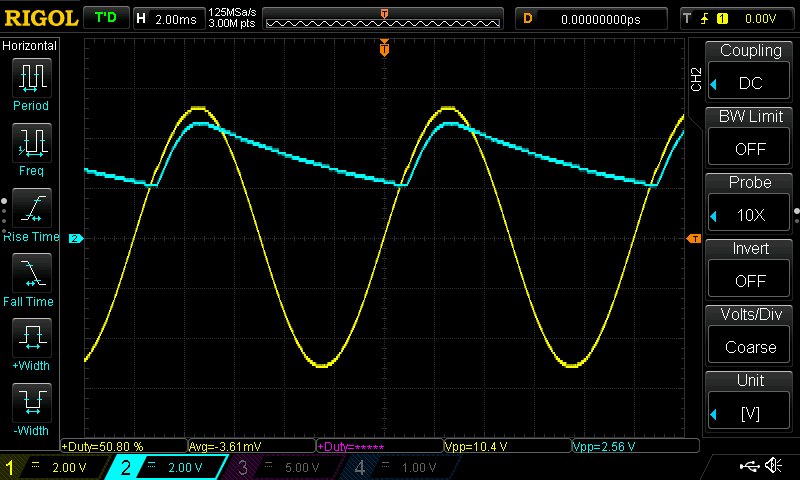
\includegraphics[scale=0.2]{raddrizzatoreASempliceSemionda1micro100}
						\caption{Raddrizzatore a semplice semionda con il condensatore da $ 1 \, \mathrm{\mu F} $ e con una frequenza di $ 100 \, \mathrm{Hz} $.}
					\end{subfigure}
					\begin{subfigure}{0.4\textwidth}
						\centering
						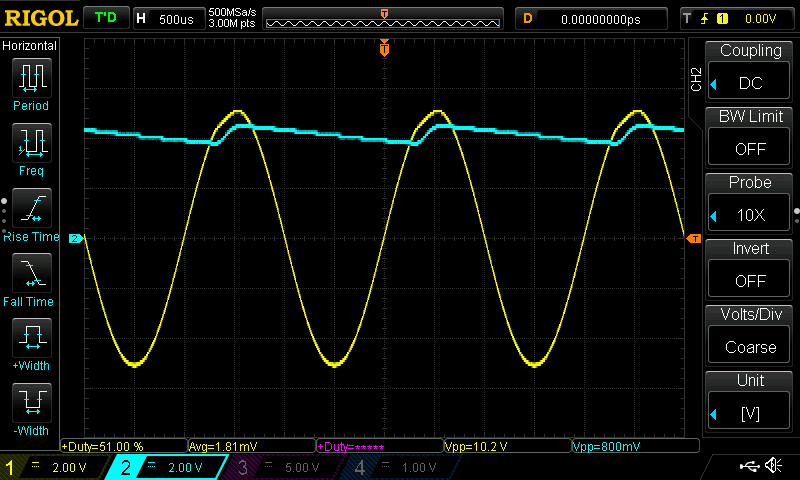
\includegraphics[scale=0.2]{raddrizzatoreASempliceSemionda1micro500}
						\caption{Raddrizzatore a semplice semionda con il condensatore da $ 1 \, \mathrm{\mu F} $ e con una frequenza di $ 500 \, \mathrm{Hz} $.}
					\end{subfigure}
					\begin{subfigure}{1\textwidth}
						\centering
						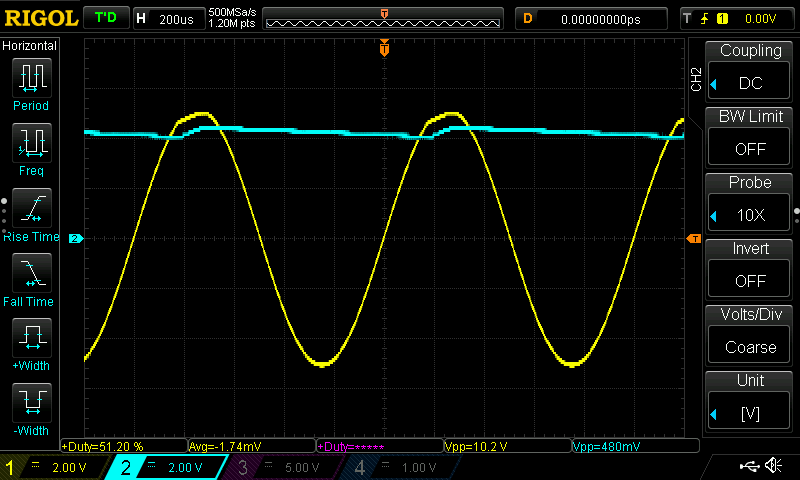
\includegraphics[scale=0.3]{raddrizzatoreASempliceSemionda1micro1k}
						\caption{Raddrizzatore a semplice semionda con il condensatore da $ 1 \, \mathrm{\mu F} $ e con una frequenza di $ 1 \, \mathrm{kHz} $.}
					\end{subfigure}
					\label{fig:raddrizzatoreASempliceSemionda1micro}
				\end{figure}
				\newpage
		\subsection{Circuito per la protezione da scariche elettrostatiche}
			\begin{center}
				$ V_{\mathrm{min}}= -600 \, \mathrm{mV} $
			\end{center}
			\newline
			\begin{center}
				$ V_{\mathrm{max}}= 6.00 \, \mathrm{V} $
			\end{center}
\end{document}